\newpage
\chapter{Частица в кулоновом поле. Уровни энергии и волновые функции}
\par Рассмотрим потенциал вида $U=-\alpha/r$, где $\alpha>0$. Для атома водорода $\alpha=E^2$. //куча слов о том, что невозможно отличить электроны друг от друга и про волновую функцию//
\par Запишем уравнение в таком потенциале (вывод см. в предыдущем билете):
$$R^{\prime \prime}_{kr} + \frac{2}{r}R^\prime _{r}  - \frac{l(l+1)}{r^2} R  +\frac{2m}{\hbar^2}\left( E+\frac{\alpha}{r}\right)R=0$$
\par Введем переменные для длины, времени и энергии для обезразмеривания уравнения: $L = \frac{\hbar^2}{m\alpha}$, $t=\frac{\hbar^2}{m\alpha^2}$, $[E] = \frac{m\alpha^2}{\hbar^2}$. Получим:
$$R^{\prime \prime}_{rr}+ \frac{2}{r}R^\prime _{r}   - \frac{l(l+1)}{r^2} R + 2\left(E+\frac{1}{r} \right)R $$
\par Пусть еще $r = \frac{1}{\sqrt{-2E}}$ и $\rho = \frac{2r}{n}$:
$$R^{\prime \prime} +\frac{2}{\rho} R^\prime + \left(-\frac{1}{4} + \frac{n}{\rho}-\frac{l(l+1)}{\rho^2} \right)R=0$$

\par \begin{wrapfigure}[15]{r}{0.5\linewidth} 
\vspace{-2ex}
\centering
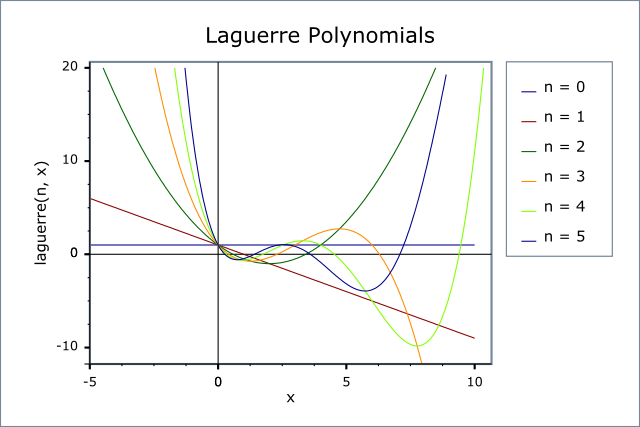
\includegraphics[width=1\linewidth]{pictures/29.1.png}
\caption{Полиномы Лагерра}
\end{wrapfigure}
\par Асимптотики: $\rho \rightarrow \infty$ и $R^{\prime \prime} -\frac{1}{4} R=0$, а значит, решение $R\rightarrow e^{-\rho/2}$ (знак выбран таким образом, что все затухает на бесконечности);$\rho \rightarrow 0$, попробуем подстановку $R=\rho^2 e^{-\rho/2} W(\rho)$:
$$\rho W^{\prime \prime} +(2l+2-\rho)W^\prime +(n-l-1)W =0$$
\par Решением являются спец-функции - \textbf{полиномы Лагерра}, причем должно выполняться условие $(n-l-1)\geq 0$, $n \in \mathds{Z}$. Получили энергию $E=-\frac{m \alpha^2}{2\hbar^2 n^2}$ с нижней границей $n \geq l+1$ , которая определяет \textbf{главное квантовое число}, связанное с  с радиальным и орбитальным квантовыми числами: $n_г = n-l-1$, оно равно числу узлов радиальной части волновой функции. Для любого n есть вырождение. //явно что-то говорил в этом месте//
\par Еще какие-то замечания, числа, формулы:
$\frac{\hbar^2}{ml^2}=0.8 \cdot 10^{-8} cm$ - пол-Ангстрема, боровский радиус;
$\frac{me^4}{\hbar^2}=27.21 эВ$ - масштаб/глубина энергии;
Число Ридберга - $R_y = 0.5 \frac{me^4}{\hbar^2}$
\par Число вырождения уровня при заданном $n$ и при $l=\{ 0,1,2,...,n-1\}$ равно $\sum^{n-1}_{l=0} (2l+1)=n^2$.